\documentclass[varwidth=\maxdimen]{standalone}
\usepackage{pgfplots}
\usepackage{pgfplotstable}
\usepackage{tikz}
\usetikzlibrary{
  decorations.pathreplacing,
  calc,
  decorations.fractals,
  through,
  shapes,
  patterns,
  arrows.meta,
  arrows,
  calligraphy,
  shapes.symbols,
  shapes.geometric,
  patterns,
  matrix,
  fit
}
\usepackage{amsmath}
\usepackage{amsfonts}
\usepackage{xfrac}
\usepackage{xcolor}
% \usepackage{xr}
\usepackage{mathtools}
\usepackage{xr-hyper}
\usepackage{hyperref}
\externaldocument{Invariant_Measure_SHE_JPT_Revision}
\newcommand\R{\mathbb{R}}

\begin{document}
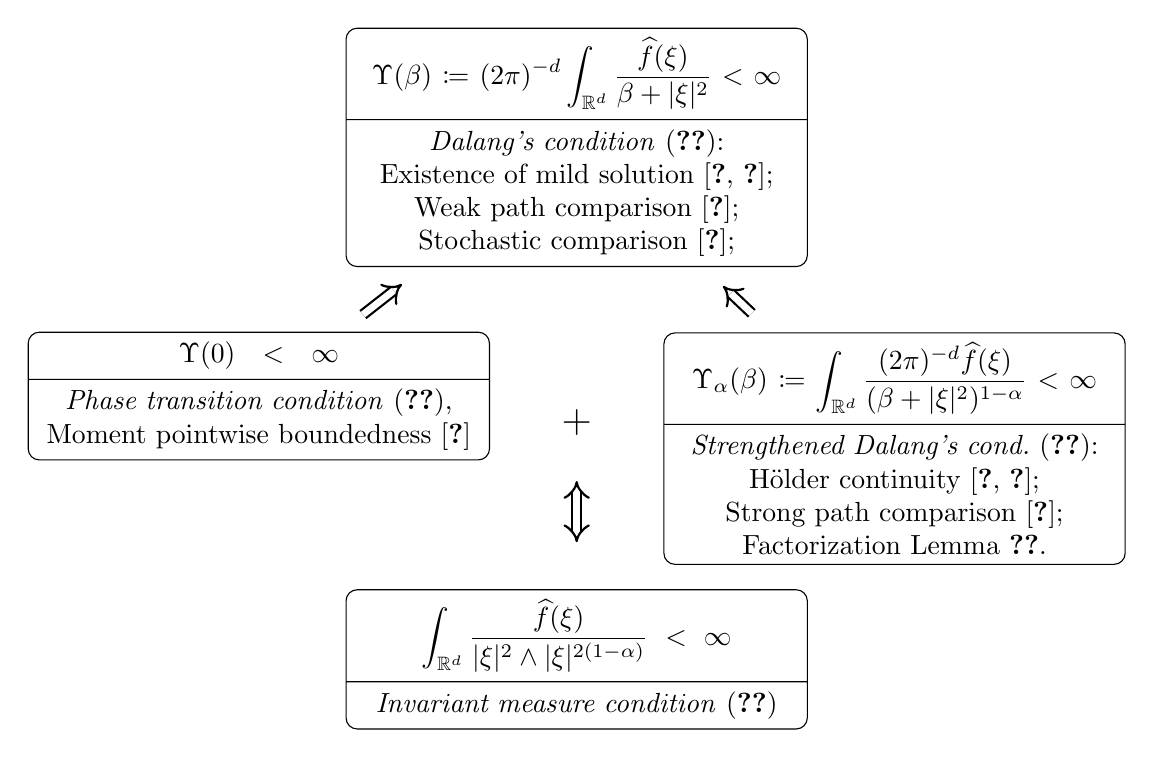
\begin{tikzpicture}
    [node distance = 12em, >=stealth, auto]
		% \tikzset{> = latex}
    % \tikzset{MyNodeStyle/.style={align = center, draw, rounded corners = 0.5em}}
    % \tikzset{MyImplies/.style={
    %     -Implies,
    %     line width = 0.8pt,
    %     double distance = 3.5pt,
    %     shorten >= 15pt,
    %     shorten <= 15pt,
    %   }}

    \tikzset{
      MyImplies/.style={
        -Implies,
        line width = 0.8pt,
        double distance = 2.5pt,
        shorten >= 10pt,
        shorten <= 10pt,
      },
      MyNode/.style={
        draw,
        rectangle split,
        rectangle split parts = 2,
        text centered,
        text width = 16em,
        rounded corners,
      },
    }

    \node[MyNode] (Dalang)
      {$\displaystyle \Upsilon(\beta) \coloneqq (2\pi)^{-d} \int_{\mathbb{R}^d} \frac{\widehat{f}(\ud \xi)}{\beta+|\xi|^2}<\infty$
        \nodepart{second}
          \textit{Dalang's condition} \eqref{E:Dalang}:\\
          Existence of mild solution \cite{dalang:99:extending,chen.kim:19:nonlinear};
          Weak path comparison~\cite{chen.huang:19:comparison};
          Stochastic comparison~\cite{chen.kim:20:stochastic};
    };

		\node[below right of = Dalang, MyNode, xshift = 3em, yshift = -2.4em] (Factor)
      {$\displaystyle \Upsilon_\alpha(\beta) \coloneqq \int_{\mathbb{R}^d} \frac{(2\pi)^{-d} \widehat{f}(\ud \xi)}{(\beta+|\xi|^2)^{1-\alpha}}<\infty$
        \nodepart{second}
          \textit{Strengthened Dalang's cond.}~\eqref{E:Dalang-ab}:\\
          H\"older continuity~\cite{sanz-sole.sarra:02:holder,chen.huang:19:comparison}; \\
          Strong path comparison~\cite{chen.huang:19:comparison}; \\
          Factorization Lemma~\ref{L:Factorize}.
    };
		\node[below left of = Dalang, MyNode, xshift = -3em, yshift = -0.5em] (Phase)
      {$\Upsilon(0)<\infty$
        \nodepart{second}
          \textit{Phase transition condition}~\eqref{E:Dalang-00},\\
          Moment pointwise boundedness~\cite{chen.kim:19:nonlinear}
      };

    \node (Plus) at ($(Factor)!0.5!(Phase)$) {\Large $+$};

    \node[below of = Dalang, yshift = -6.5em, MyNode] (Inv)
      {$\displaystyle \int_{\R^d} \frac{\widehat{f}(\ud \xi)}{|\xi|^2\wedge|\xi|^{2(1-\alpha)}}<\infty$
        \nodepart{second}
          \textit{Invariant measure condition}~\eqref{E:SpectralCond}
    };

    \draw[MyImplies] (Factor) -- (Dalang);
    \draw[MyImplies] (Phase) -- (Dalang);
    \draw[MyImplies,
        shorten >= 17pt,
        shorten <= 17pt,
      ] (Plus) -- (Inv);
    \draw[MyImplies,
        shorten >= 13pt,
        shorten <= 30pt,
      ] (Inv) -- (Plus);

\end{tikzpicture}
\end{document}
